% Figure 1: the reservoir, the jump families, dark-state protection and what an old input becomes.
% Build: pdflatex fig1_concept.tex -> fig1_concept.pdf, drawn at the text width of the Quantum class (17 cm).
\documentclass[tikz,border=0pt]{standalone}
\usepackage[scaled=0.95]{helvet}
\renewcommand{\familydefault}{\sfdefault}
\usepackage{amsmath}
\usepackage{sansmath}
\sansmath
\DeclareMathSymbol{-}{\mathbin}{operators}{123}
\usetikzlibrary{arrows.meta,decorations.pathmorphing,calc}
\definecolor{ink}{HTML}{1A1A1A}
\definecolor{ink2}{HTML}{3A3A3A}
\definecolor{ink3}{HTML}{6F6F6F}
\definecolor{local}{HTML}{C8553D}
\definecolor{exch}{HTML}{C9852A}
\definecolor{deph}{HTML}{6B7385}
\definecolor{pair}{HTML}{2A9D8F}
\definecolor{shared}{HTML}{16325C}
\definecolor{input}{HTML}{7B5EA7}
\definecolor{strong}{HTML}{9C6644}
\definecolor{gentle}{HTML}{2D6A4F}
\definecolor{env}{HTML}{A89F91}
\definecolor{dot}{HTML}{CFCFCF}
\begin{document}
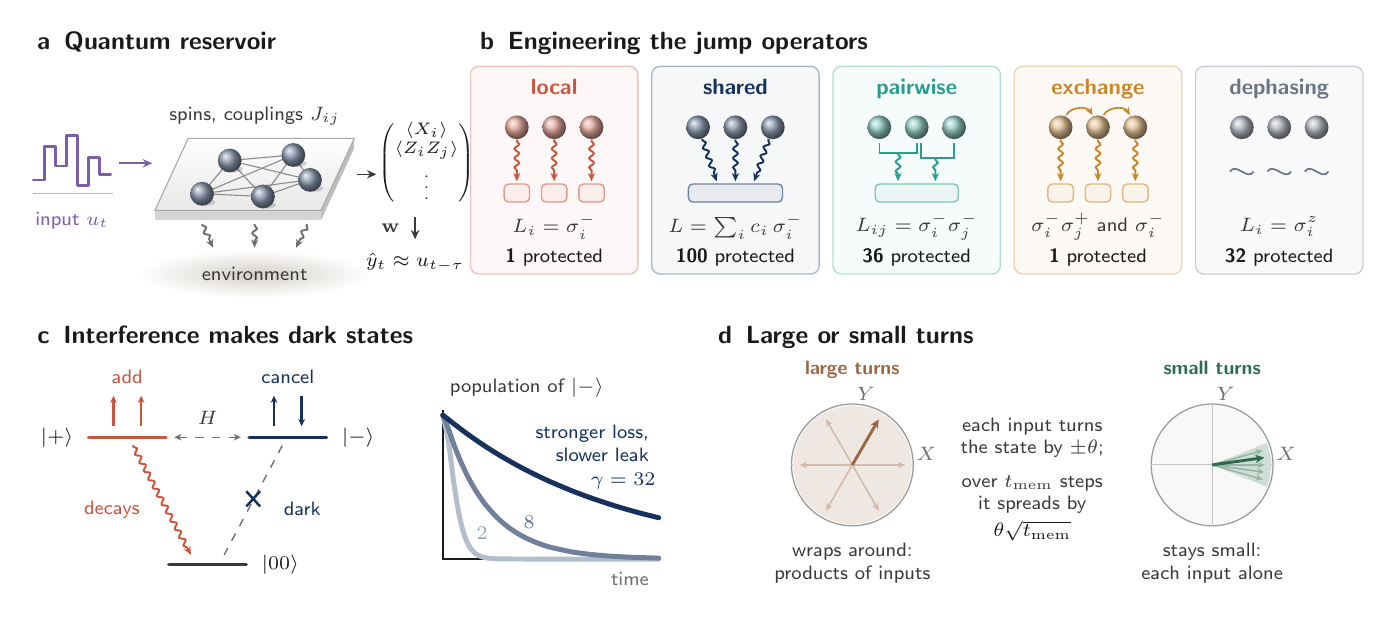
\begin{tikzpicture}[x=1pt,y=1pt,
  font=\fontsize{7.4}{8.8}\selectfont, text=ink,
  ttl/.style={anchor=base west,font=\fontsize{8.6}{10.3}\selectfont\bfseries},
  head/.style={anchor=base,font=\fontsize{7.8}{9}\selectfont\bfseries},
  small/.style={font=\fontsize{7}{8.2}\selectfont},
  tiny/.style={font=\fontsize{6.6}{7.6}\selectfont},
  spin/.style={circle,minimum size=8.6pt,inner sep=0pt,shading=ball,ball color=#1!50!white},
  spin/.default=shared,
  bath/.style={rounded corners=1.6pt,fill=#1!10,draw=#1!60,line width=0.5pt},
  card/.style={rounded corners=3pt,fill=#1!4,draw=#1!35,line width=0.5pt},
  decay/.style={-{Stealth[length=3pt,width=2.6pt]},#1,line width=0.7pt,
    decorate,decoration={snake,amplitude=0.85pt,segment length=3.4pt,pre length=0.5pt,post length=2.4pt}},
  link/.style={ink3!80,line width=0.4pt},
  arr/.style={-{Stealth[length=3.4pt,width=3pt]},ink2,line width=0.6pt},
  lvl/.style={line width=1.2pt,line cap=round,#1},
  mix/.style={{Stealth[length=2.6pt,width=2.4pt]}-{Stealth[length=2.6pt,width=2.4pt]},ink3,dashed,line width=0.5pt},
  hot/.style={circle,inner sep=0pt,minimum size=4.8pt,fill=#1},
  cold/.style={circle,inner sep=0pt,minimum size=3.2pt,fill=dot},
  plus/.style={rectangle,inner sep=0pt,minimum size=5pt,fill=input!75,draw=input!75,line width=0.5pt},
  minus/.style={rectangle,inner sep=0pt,minimum size=5pt,fill=white,draw=input!75,line width=0.5pt},
]
\path[use as bounding box] (0,0) rectangle (483.7,206);

%=================================================================== a  the reservoir
\node[ttl] at (0,198) {a\hspace{0.5em}Quantum reservoir};
% input stream
\draw[ink3!50,line width=0.4pt] (2,146) -- (31,146);
\draw[input,line width=0.95pt,line join=round,line cap=round]
  (2,151) -- (6,151) -- (6,163) -- (10,163) -- (10,156) -- (14,156) -- (14,167) -- (18,167)
  -- (18,149) -- (22,149) -- (22,159) -- (26,159) -- (26,153) -- (30,153);
\node[anchor=north,text=input,small] at (16,143) {input $u_t$};
\draw[-{Stealth[length=3.4pt,width=3pt]},input,line width=0.7pt] (33,157) -- (45,157);
% spin platform in perspective
\fill[ink3!30] (46,140) -- (106,140) -- (106,136.4) -- (46,136.4) -- cycle;
\fill[ink3!45] (106,140) -- (118,166) -- (118,162.4) -- (106,136.4) -- cycle;
\shade[top color=white,bottom color=ink3!16] (46,140) -- (106,140) -- (118,166) -- (58,166) -- cycle;
\draw[ink3!60,line width=0.4pt] (46,140) -- (106,140) -- (118,166) -- (58,166) -- cycle;
\coordinate (s1) at (63,146); \coordinate (s2) at (85,145); \coordinate (s3) at (102,151);
\coordinate (s4) at (73,158); \coordinate (s5) at (96,160);
\foreach \a/\b in {1/2,1/3,1/4,1/5,2/3,2/4,2/5,3/4,3/5,4/5}{\draw[link] (s\a) -- (s\b);}
\foreach \k in {1,...,5}{\fill[black,opacity=0.16] ($(s\k)+(1.3,-3.1)$) ellipse (3.5pt and 1.2pt);}
\foreach \k in {1,...,5}{\node[spin] at (s\k) {};}
\node[small,text=ink2] at (82,174) {spins, couplings $J_{ij}$};
% environment
\shade[inner color=env!50,outer color=white] (82,117) ellipse (42pt and 8.5pt);
\node[small,text=ink2] at (82,117) {environment};
\draw[decay=ink3] (63,135) -- (67,126.5);
\draw[decay=ink3] (82,135) -- (82,126.5);
\draw[decay=ink3] (101,135) -- (97,126.5);
% linear readout
\draw[arr] (119,153) -- (126,153);
\node[anchor=west,inner sep=0pt,font=\fontsize{5.9}{6.8}\selectfont] (x) at (126.5,157)
  {$\begin{pmatrix}\langle X_i\rangle\\ \langle Z_iZ_j\rangle\\ \vdots\end{pmatrix}$};
\draw[arr] (140,137.5) -- (140,129.5);
\node[anchor=east,small,text=ink2] at (138,133.5) {$\mathbf w$};
\node[anchor=north,small] at (140,128) {$\hat y_t\approx u_{t-\tau}$};

%=================================================================== b  jump families
\node[ttl] at (160,198) {b\hspace{0.5em}Engineering the jump operators};
\newcommand{\trio}[3]{%
  \node[spin=#3] (#1a) at (#2-13.5,170) {};
  \node[spin=#3] (#1b) at (#2,170) {};
  \node[spin=#3] (#1c) at (#2+13.5,170) {};}
\foreach \x/\c in {160/local,225.5/shared,291/pair,356.5/exch,422/deph}{\draw[card=\c] (\x,117) rectangle ++(60.5,75);}
% local
\node[head,text=local] at (190.25,182) {local};
\trio{L}{190.25}{local}
\foreach \x in {176.75,190.25,203.75}{\draw[bath=local] (\x-4.6,143) rectangle (\x+4.6,149.5);}
\foreach \n/\x in {a/176.75,b/190.25,c/203.75}{\draw[decay=local] (L\n) -- (\x,150.5);}
\node[text=ink2] at (190.25,134) {$L_i=\sigma_i^-$};
\node at (190.25,123) {\textbf{1} protected};
% shared
\node[head,text=shared] at (255.75,182) {shared};
\trio{S}{255.75}{shared}
\draw[bath=shared] (238.75,143) rectangle (272.75,149.5);
\draw[decay=shared] (Sa) -- (249,150.5);
\draw[decay=shared] (Sb) -- (255.75,150.5);
\draw[decay=shared] (Sc) -- (262.5,150.5);
\node[text=ink2] at (255.75,134) {$L=\sum_i c_i\,\sigma_i^-$};
\node at (255.75,123) {\textbf{100} protected};
% pairwise
\node[head,text=pair] at (321.25,182) {pairwise};
\trio{P}{321.25}{pair}
\draw[pair,line width=0.6pt] ($(Pa)+(0,-5.8)$) -- ++(0,-3.4) -| ($(Pb)+(0,-5.8)$);
\draw[pair,line width=0.6pt] ($(Pb)+(1.5,-5.8)$) -- ++(0,-5.4) -| ($(Pc)+(0,-5.8)$);
\draw[bath=pair] (306.25,143) rectangle (336.25,149.5);
\draw[decay=pair] (314.5,160.8) -- (314.5,150.5);
\draw[decay=pair] (328,158.8) -- (328,150.5);
\node[text=ink2] at (321.25,134) {$L_{ij}=\sigma_i^-\sigma_j^-$};
\node at (321.25,123) {\textbf{36} protected};
% exchange
\node[head,text=exch] at (386.75,182) {exchange};
\trio{E}{386.75}{exch}
\draw[-{Stealth[length=2.8pt,width=2.4pt]},exch,line width=0.6pt] ($(Ea)+(2,4.4)$) to[bend left=60] ($(Eb)+(-2,4.4)$);
\draw[-{Stealth[length=2.8pt,width=2.4pt]},exch,line width=0.6pt] ($(Eb)+(2,4.4)$) to[bend left=60] ($(Ec)+(-2,4.4)$);
\foreach \x in {373.25,386.75,400.25}{\draw[bath=exch] (\x-4.6,143) rectangle (\x+4.6,149.5);}
\foreach \n/\x in {a/373.25,b/386.75,c/400.25}{\draw[decay=exch] (E\n) -- (\x,150.5);}
\node[text=ink2] at (386.75,134) {$\sigma_i^-\sigma_j^+$ and $\sigma_i^-$};
\node at (386.75,123) {\textbf{1} protected};
% dephasing
\node[head,text=deph] at (452.25,182) {dephasing};
\trio{D}{452.25}{deph}
\foreach \x in {438.75,452.25,465.75}{
  \draw[deph,line width=0.6pt] (\x-4.3,154) .. controls (\x-2,157.5) and (\x+2,150.5) .. (\x+4.3,154);}
\node[text=ink2] at (452.25,134) {$L_i=\sigma_i^z$};
\node at (452.25,123) {\textbf{32} protected};

%=================================================================== c  interference and the Zeno effect
\node[ttl] at (0,92) {c\hspace{0.5em}Interference makes dark states};
% two spins sharing one channel: |+> and |-> above |00>
\draw[lvl=local] (22,58) -- (50,58);
\node[anchor=east,small] at (20,58) {$|{+}\rangle$};
\draw[lvl=shared] (80,58) -- (108,58);
\node[anchor=west,small] at (110,58) {$|{-}\rangle$};
\draw[lvl=ink2] (51,12) -- (79,12);
\node[anchor=west,small] at (81,12) {$|00\rangle$};
% the decay amplitudes of |10> and |01> add or cancel
\foreach \x in {31,41}{\draw[-{Stealth[length=2.6pt,width=2.4pt]},local,line width=0.85pt] (\x,62) -- (\x,73);}
\node[anchor=south,tiny,text=local] at (36,74) {add};
\draw[-{Stealth[length=2.6pt,width=2.4pt]},shared,line width=0.85pt] (89,62) -- (89,73);
\draw[-{Stealth[length=2.6pt,width=2.4pt]},shared,line width=0.85pt] (99,73) -- (99,62);
\node[anchor=south,tiny,text=shared] at (94,74) {cancel};
% decay of the bright state, none of the dark state
\draw[decay=local] (38,55) -- (59,15.5);
\node[anchor=east,small,text=local] at (44,32) {decays};
\draw[ink3,dashed,line width=0.5pt] (92,55) -- (71,15.5);
\draw[shared,line width=0.9pt] (79,33) -- (84,38.5) (79,38.5) -- (84,33);
\node[anchor=west,small,text=shared] at (89,32) {dark};
\draw[mix] (53,58) -- (77,58);
\node[anchor=south,small,text=ink2] at (65,59) {$H$};
% inset: survival of the dark state, two spins with coupling H = g and shared loss gamma (time in 1/g)
\begin{scope}[shift={(150,14)}]
  \draw[ink,line width=0.8pt] (0,54) -- (0,0) -- (78,0);
  \node[anchor=north east,tiny,text=ink3] at (78,-1.2) {time};
  \node[anchor=south west,tiny,text=ink2] at (-1,55) {population of $|{-}\rangle$};
  \begin{scope}[x=78pt,y=52pt]
    \draw[shared!32,line width=1.8pt,line cap=round] plot[smooth] coordinates {(0.000,1.0000) (0.025,0.8277) (0.050,0.5413) (0.075,0.3112) (0.100,0.1648) (0.125,0.0825) (0.150,0.0397) (0.175,0.0185) (0.200,0.0084) (0.225,0.0037) (0.250,0.0016) (0.300,0.0003) (0.400,0.0000) (0.600,0.0000) (0.800,0.0000) (1.000,0.0000)};
    \draw[shared!62,line width=1.8pt,line cap=round] plot[smooth] coordinates {(0.000,1.0000) (0.025,0.9092) (0.050,0.8013) (0.075,0.7057) (0.100,0.6216) (0.125,0.5474) (0.150,0.4821) (0.175,0.4246) (0.200,0.3740) (0.250,0.2901) (0.300,0.2250) (0.350,0.1745) (0.400,0.1354) (0.450,0.1050) (0.500,0.0814) (0.600,0.0490) (0.700,0.0295) (0.800,0.0177) (0.900,0.0107) (1.000,0.0064)};
    \draw[shared,line width=1.8pt,line cap=round] plot[smooth] coordinates {(0.000,1.0000) (0.050,0.9412) (0.100,0.8841) (0.150,0.8305) (0.200,0.7801) (0.250,0.7328) (0.300,0.6884) (0.350,0.6466) (0.400,0.6074) (0.450,0.5706) (0.500,0.5360) (0.600,0.4729) (0.700,0.4173) (0.800,0.3682) (0.900,0.3249) (1.000,0.2867)};
  \end{scope}
  \node[anchor=south west,tiny,text=shared!45,inner sep=1pt] at (11,6) {$2$};
  \node[anchor=south west,tiny,text=shared!70,inner sep=1pt] at (28,10) {$8$};
  \node[anchor=south east,tiny,text=shared,inner sep=1pt] at (78,24) {$\gamma=32$};
  \node[anchor=north east,small,text=shared,align=right] at (78,52) {stronger loss,\\slower leak};
\end{scope}

%=================================================================== d  strong or gentle writing
\node[ttl] at (246,92) {d\hspace{0.5em}Large or small turns};
\newcommand{\bloch}[1]{%
  \fill[ink3!5] #1 circle (22pt);
  \draw[ink3!70,line width=0.45pt] #1 circle (22pt);
  \draw[ink3!40,line width=0.35pt] ($#1+(-22pt,0)$) -- ($#1+(22pt,0)$);
  \draw[ink3!40,line width=0.35pt] ($#1+(0,-22pt)$) -- ($#1+(0,22pt)$);
  \node[tiny,text=ink3,anchor=south west,inner sep=1pt] at ($#1+(0.5pt,22pt)$) {$Y$};
  \node[tiny,text=ink3,anchor=south west,inner sep=1pt] at ($#1+(22pt,0.3pt)$) {$X$};}
\tikzset{vec/.style={-{Stealth[length=2.6pt,width=2.4pt]},line width=0.55pt},
         bold/.style={-{Stealth[length=3.2pt,width=3pt]},line width=1.05pt}}
% strong: the direction spreads over the whole circle
\bloch{(298,48)}
\fill[strong!16] (298,48) circle (21.3pt);
\foreach \a in {0,60,120,180,240,300}{\draw[vec,strong!45] (298,48) -- ++(\a:19pt);}
\draw[bold,strong] (298,48) -- ++(60:19pt);
\node[anchor=base,font=\fontsize{7.2}{8.4}\selectfont\bfseries,text=strong] at (298,80.5) {large turns};
\node[anchor=base,small,text=ink2] at (298,15) {wraps around:};
\node[anchor=base,small,text=ink2] at (298,6.5) {products of inputs};
% gentle: the direction stays in a narrow fan
\bloch{(428,48)}
\fill[gentle!22] (428,48) -- ++(-22:21.3pt) arc[start angle=-22,end angle=22,radius=21.3pt] -- cycle;
\foreach \a in {-16,-8,0,8,16}{\draw[vec,gentle!50] (428,48) -- ++(\a:19pt);}
\draw[bold,gentle] (428,48) -- ++(8:19pt);
\node[anchor=base,font=\fontsize{7.2}{8.4}\selectfont\bfseries,text=gentle] at (428,80.5) {small turns};
\node[anchor=base,small,text=ink2] at (428,15) {stays small:};
\node[anchor=base,small,text=ink2] at (428,6.5) {each input alone};
% the rule in between
\node[anchor=base,small,text=ink2] at (363,60) {each input turns};
\node[anchor=base,small,text=ink2] at (363,52) {the state by $\pm\theta$;};
\node[anchor=base,small,text=ink2] at (363,40) {over $t_{\mathrm{mem}}$ steps};
\node[anchor=base,small,text=ink2] at (363,32) {it spreads by};
\node[anchor=base,small,text=ink] at (363,22) {$\theta\sqrt{t_{\mathrm{mem}}}$};
\end{tikzpicture}
\end{document}
